%%%%%%%%%%%%%%%%%%%%%%%%%%%%%%%%%%%%%%%%%%%%%%%%%%%%%%%%%%%%%%%%%%%%%%%%%%%%%%%%%%%%%%%%%%%%%%%%%%%%%%%%%%%%%%%%%%%%%%%%%%%%%%%%%%%%%%%%%%%%%%%%%%%%%%%%%%%
% This is just an example/guide for you to refer to when submitting manuscripts to Frontiers, it is not mandatory to use Frontiers .cls files nor frontiers.tex  %
% This will only generate the Manuscript, the final article will be typeset by Frontiers after acceptance.   
%                                              %
%                                                                                                                                                         %
% When submitting your files, remember to upload this *tex file, the pdf generated with it, the *bib file (if bibliography is not within the *tex) and all the figures.
%%%%%%%%%%%%%%%%%%%%%%%%%%%%%%%%%%%%%%%%%%%%%%%%%%%%%%%%%%%%%%%%%%%%%%%%%%%%%%%%%%%%%%%%%%%%%%%%%%%%%%%%%%%%%%%%%%%%%%%%%%%%%%%%%%%%%%%%%%%%%%%%%%%%%%%%%%%

%%% Version 3.4 Generated 2022/06/14 %%%
%%% You will need to have the following packages installed: datetime, fmtcount, etoolbox, fcprefix, which are normally inlcuded in WinEdt. %%%
%%% In http://www.ctan.org/ you can find the packages and how to install them, if necessary. %%%
%%%  NB logo1.jpg is required in the path in order to correctly compile front page header %%%

\documentclass[utf8]{FrontiersinVancouver}

\usepackage{url,hyperref,lineno,microtype}
\usepackage[onehalfspacing]{setspace}
\usepackage[version=4]{mhchem} % for element symbols
\usepackage{wasysym} % for diameter symbol
\usepackage{multirow}
\usepackage{threeparttable}
%\usepackage{subcaption}	% will use only figures with built-in subfigures for automatic numbering of figure order

% Raise version of output document to 1.7 ti suppress warning
% PDF inclusion: found PDF version <1.7> but at most version <1.5> allowed
\pdfminorversion=7

\linenumbers

% Leave a blank line between paragraphs instead of using \\


\def\keyFont{\fontsize{8}{11}\helveticabold}
\def\firstAuthorLast{Strugari {et~al.}} %use et al only if is more than 1 author

\def\Authors{Matthew Strugari\,$^{1,2,*}$, Carles Falcon\,$^{3}$, Kjell Erlandsson\,$^{4}$, Brian Hutton\,$^{4}$, Kimberly Brewer\,$^{1,2,5}$, and Kris Thielemans\,$^{4}$}
% Affiliations should be keyed to the author's name with superscript numbers and be listed as follows: Laboratory, Institute, Department, Organization, City, State abbreviation (USA, Canada, Australia), and Country (without detailed address information such as city zip codes or street names).
% If one of the authors has a change of address, list the new address below the correspondence details using a superscript symbol and use the same symbol to indicate the author in the author list.

\def\Address{
$^{1}$Biomedical MRI Research Laboratory, IWK Health Centre, Halifax, Canada\\
$^{2}$Department of Physics \&  Atmospheric Science, Dalhousie University, Halifax, Canada\\
$^{3}$Neuroimaging Group, Barcelona$\mathrm{\beta}$eta Brain Research Center, Barcelona, Spain\\
$^{4}$Institute of Nuclear Medicine, University College London, London, UK\\
$^{5}$Department of Diagnostic Radiology, Dalhousie University, Halifax, Canada
}
% The Corresponding Author should be marked with an asterisk
% Provide the exact contact address (this time including street name and city zip code) and email of the corresponding author
\def\corrAuthor{Matthew Strugari}
\def\corrEmail{matthew.strugari@dal.ca}






\begin{document}
\onecolumn
\firstpage{1}

\title[Pinhole-SPECT reconstruction with STIR]{Integration of advanced 3D SPECT modelling for pinhole collimators into the open-source STIR framework} 

\author[\firstAuthorLast ]{\Authors} %This field will be automatically populated
\address{} %This field will be automatically populated
\correspondance{} %This field will be automatically populated

\extraAuth{}% If there are more than 1 corresponding author, comment this line and uncomment the next one.
%\extraAuth{corresponding Author2 \\ Laboratory X2, Institute X2, Department X2, Organization X2, Street X2, City X2 , State XX2 (only USA, Canada and Australia), Zip Code2, X2 Country X2, email2@uni2.edu}


\maketitle

\begin{abstract}

%%% Leave the Abstract empty if your article does not require one, please see the Summary Table for full details.
\section{}
Pinhole-SPECT systems are becoming increasingly important in clinical and preclinical nuclear medicine investigations as they can provide a superior resolution-sensitivity tradeoff compared to conventional parallel-hole and fan-beam collimators. Previously, open-source software did not exist for reconstructing tomographic images from pinhole-SPECT datasets. A 3D SPECT system matrix modelling library specific for pinhole collimators has recently been integrated into STIR --- an open-source software package for tomographic image reconstruction. The pinhole-SPECT library enables corrections for attenuation and the spatially variant collimator-detector response by incorporating their effects into the system matrix. Attenuation corrections can be calculated with a simple single line-of-response or a full model. The spatially variant collimator-detector response can be modelled with point spread function and depth of interaction corrections for increased system matrix accuracy. Improvements to computational speed and memory requirements can be made with image masking. This work demonstrates the flexibility and accuracy of STIR's forthcoming support for pinhole-SPECT datasets using measured and simulated single-pinhole SPECT data from which reconstructed images were analyzed quantitatively and qualitatively. The extension of the open-source STIR project with advanced pinhole-SPECT modelling will enable the research community to study the impact of pinhole collimators in several SPECT imaging scenarios and with different scanners.

%Pinhole-SPECT systems are becoming increasingly important in preclinical and clinical nuclear medicine investigations as they can provide a superior resolution-sensitivity tradeoff compared to conventional parallel-hole and fan-beam collimators. Previously, open-source software did not exist for reconstructing tomographic images from pinhole-SPECT datasets. A 3D SPECT system matrix modelling library specific for pinhole collimators has recently been integrated into STIR --- an open-source software package for tomographic image reconstruction --- and made accessible from SIRF --- an open-source software package targeting synergistic image reconstruction. The pinhole-SPECT library enables corrections for attenuation and the spatially variant collimator-detector response by incorporating their effects into the system matrix. Attenuation corrections can be calculated with a simple single line-of-response or a full model. The spatially variant collimator-detector response can be modelled with point spread function and depth of interaction corrections for increased system matrix accuracy. Improvements to computational speed and memory requirements can be made with image masking. This work demonstrates the flexibility and accuracy of STIR's and SIRF's forthcoming support for pinhole-SPECT datasets using measured and simulated data from which reconstructed images were analyzed quantitatively and qualitatively. The extension of the open-source STIR and SIRF projects with advanced pinhole-SPECT modelling will enable the research community to study the impact of pinhole collimators in several SPECT imaging scenarios and with different scanners while exploring the benefits of synergistic multi-modality reconstruction.


\tiny
 \keyFont{ \section{Keywords:} Image reconstruction, molecular imaging, Monte Carlo methods, nuclear medicine, SPECT} 
 %All article types: you may provide up to 8 keywords; at least 5 are mandatory.
\end{abstract}

\section{Introduction}

Single-photon emission computed tomography (SPECT) is based on the detection of individual $\gamma$-rays emitted from a radiotracer distribution within a subject. An Anger camera detects the $\gamma$-rays with a scintillating crystal and associated electronics after they have passed through a collimator. The collimator acts as a lens to form a 2D projection image identifying the direction from which the $\gamma$-rays originated, and a series of projection images acquired from different angles can be subsequently used to reconstruct the 3D radiotracer distribution in a tomographic image. 

The design of the collimator in terms of hole-size, material, and overall geometry, among other factors, affects the spatial resolution and sensitivity of a SPECT system. A number of designs exist including but not limited to parallel-hole, fan-beam, converging and diverging, slit-slat, coded-aperture, and single- and multi-pinhole collimators. Therefore, the choice of collimator design is application dependent in order to channel photons of different energies, magnify or minify images, or select between imaging quality and imaging speed~\citep{van_mullekom_group_collimators_2021}. Although parallel-hole and fan-beam collimators are conventionally used when imaging small fields-of-view (FOVs), pinhole collimators can provide a superior resolution-sensitivity tradeoff~\citep{islamian_advances_2015}. Besides the successful application of pinhole-SPECT systems in small-animal imaging, there has been a resurgence in the use of pinhole collimators for clinical cardiac and brain studies and when imaging small FOVs~\citep{ozsahin_clinical_2020}.

While the use of pinhole-SPECT has regained popularity in clinical and preclinical investigations of molecular imaging agents, there are no open-source software solutions available for reconstructing pinhole-SPECT datasets.  However, recent efforts have led to the integration of a 3D SPECT system matrix modelling library for pinhole collimators into the open-source Software for Tomographic Image Reconstruction (STIR). The STIR package is an object-oriented library implemented in C++ that provides a framework for research in the processing and reconstruction of emission tomography studies~\citep{thielemans_stir_2012}. Initially written for support of positron emission tomography (PET) data, STIR was previously extended to handle SPECT data with parallel- and converging-hole collimators~\citep{marti_fuster_integration_2013, marti_fuster_evaluation_2013}. The expansion of STIR's support for pinhole collimators marks the first open-source platform for reconstructing pinhole-SPECT datasets which is important in the advancement of molecular imaging techniques and technologies. 

%More information on SIRF would go here.

This work aims to demonstrate the forthcoming capabilities of STIR's support for pinhole-SPECT datasets. This was achieved by integrating parts of the SPECT Reconstruction Library developed at the University of Barcelona (SRL-UB) into STIR~\citep{falcon_metodos_1999, cot_absolute_2005, pareto_geometrical_2002, pareto_iterative_2003}. The library enables corrections for the spatially variant collimator-detector response and attenuation by incorporating their effects into the system matrix.

\section{Technical description}

Similar to the original \texttt{SPECTUB} implementation, the new pinhole-SPECT implementation is referred to as \texttt{PinholeSPECTUB} and includes a dedicated reader for SPECT projection data in interfile format~\citep{todd-pokropek_file_1992}. The pinhole-SPECT interfile reader utilizes the projection matrix size, pixel scaling factor, and detector radius according to the face of the scintillating crystal. Calculation of the system matrix is executed with the \texttt{ProjMatrixByBinPinholeSPECTUB} projector class derived from the existing STIR \texttt{ProjMatrixByBin} class which utilizes a detector and collimator text file in addition to the usual STIR parameter file. The parameter file is a text file which uses an Interfile-like syntax. It is composed of keywords corresponding to the names of the various reconstruction and matrix parameters with the values entered next to them. A detailed description of all parameters can be found in STIR's documentation.

The detector file defines the intrinsic resolution for point spread function (PSF) corrections, scintillating crystal attributes for depth of interaction (DOI) corrections, and orbit information for the acquisition (i.e., initial angle, number of angles, angular increment, direction of rotation, and axial position with respect to the reconstructed volume). Note that only circular camera orbits are supported at this time. The collimator file defines the radius of rotation and geometry for cylindrical or polygonal collimators (i.e., the detector element exposed by the pinhole, hole position, shape, size, tilt, and acceptance angle). An illustration of the pinhole-SPECT system matrix geometry is shown in Fig.~\ref{fig:PinholeSPECTUB_coords}.

%-------------------------------------------------
\noindent \textbf{Figure~\ref{fig:PinholeSPECTUB_coords} goes here.}
%-------------------------------------------------

The system matrix weights the contribution of each image voxel along the line of response (LOR) to each detector element. For increased system matrix accuracy, corrections can be made for the spatially variant collimator-detector response function in terms of intrinsic PSF, DOI, and/or attenuation (ATT) corrections by setting the appropriate fields in the parameter file. When PSF correction is disabled, a geometrical approach is applied by considering the shadow projection of the pinhole on the detector for higher computational speed and reduced memory requirements compared to the PSF approach, but is less accurate. When PSF correction is enabled, the shadow of the hole is convolved with the PSF in detector space to account for blurring effects of the camera. Values parsed from the parameter file define the number of sigmas to consider in the PSF along with the subsampling factor to temporally reduce PSF resolution for increased calculation accuracy before downsampling the final PSF to the bin size. Furthermore, when PSF or DOI corrections are enabled, an additional parsed parameter sets the spatial resolution in which to sample PSF and DOI distributions. 

Enabling DOI corrections subdivides the scintillating crystal using Bresenham's line algorithm to calculate the crystal attenuation and DOI along the LOR. If DOI correction is disabled, then half the crystal thickness is added to the detector radius.  When ATT correction is enabled, a simple correction can be applied where the same attenuation factor is applied for the whole PSF, or a full correction can be applied where different attenuation factors are applied for each bin of the PSF~\citep{marti_fuster_evaluation_2013}. Further improvements to speed and memory can be made with image masking using the default cylinder, an attenuation map, or a mask file. The default cylinder is based on the object radius in the image volume. It is important to always set the object radius greater than or equal to the size of the object in the attenuation map or mask file when masking as the matrix weights are calculated according to this value, and failure to do so will result in an error. The projection matrix can be kept in memory or calculated per projection angle. In the latter case, the memory is released before starting calculations on a new angle, thereby reducing memory requirements but increasing computation time for iterative reconstruction algorithms.

\section{Materials and methods}

To test the pinhole-SPECT implementation in STIR, Cubresa's novel silicon-photomultiplier (SiPM)-based preclinical SPECT system --- The Spark --- was used with a single-pinhole (SPH) collimator (Cubresa Inc., Winnipeg, Canada). This system was recently characterized with the National Electrical Manufacturers Association (NEMA) NU 1-2018 Standards for Performance Measurements of Gamma Cameras, and a corresponding Geant4 Application for Tomographic Emission (GATE) Monte Carlo model was validated~\citep{strugari_nema_2022}.

Simulations and image reconstructions were performed on an HP Z820 workstation operating Ubuntu 18.04.5 LTS with two Intel Xeon E5-2630 2.3 GHz hexa-core CPUs and 64 GB of 1600 MHz DDR3 memory. The SPH-SPECT data for quantitative image assessment was simulated with GATE v9.0 while qualitative image assessment was done with \textit{in vivo} data. Tomographic images were reconstructed with STIR v5.0.2 on a single CPU core as the \texttt{PinholeSPECTUB} library has not yet been configured to use the Message Passing Interface capabilities of STIR which would allow it to perform several computations in parallel.

\subsection{Quantitative assessment of reconstructed data}



%The scanner features a 3.0 mm-thick CsI(Na) scintillator (Saint-Gobain Crystals, Hiram, USA) coupled to a 14$\times$14 SensL C-series array with 6.0 mm sensors (ON Semiconductor, Phoenix, USA) which yields a 0.85 mm intrinsic resolution. 

%The collimator radius of rotation is 28.0 mm measured to the center of the 10 mm-thick collimator face, and the detector radius of rotation is 54.75 mm measured to the face of the scintillator. Note that the rotation extent is fixed to 270~$\deg$. The system has two interchangeable tungsten collimators: a single-pinhole (SPH) collimator with a 1.0 mm hole and 90.0~$\deg$ acceptance angle, and a multiplexing multi-pinhole (MPH) collimator with five rows of 1.0 mm holes and 25.0~$\deg$ acceptance angles where each row focuses on a different volume of interest in the tomographic FOV. The SPH collimator enables an axial and transaxial tomographic FOV of 46.0 mm and 57.5 mm, respectively, and the MPH collimator FOV is 14.0 mm and 30.0 mm, respectively.

%The MPH collimator geometry was reverse-engineered from optical surface scans using an HP 3D structured light scanner to create a 3D computer model (HP Inc., Palo Alto, USA). The open-source CloudCompare package was used to register pinhole cones to the computer model to extract pinhole  geometry~\citep{cloudcompare}. Each row of pinholes was localized at approximately z~=~\{-15.0,~-7.5,~0.0,~7.5,~15.0\}~mm and focal spots were estimated to lie at the center of the tomographic FOV with transaxial focal spots at x~=~\{-5.0,~10.0,~0.0,~-10.0,~5.0\}~mm (note that the set ordering corresponds to the aforementioned rows). The pinholes were presumed to uniformly project over an 8$\times$8 cm$^2$ area located on the face of the SiPM-array. This provided necessary and sufficient information to simulate MPH-SPECT acquisitions using the new \texttt{GateParameterisedPinholeCollimator} class in GATE v9.2 to further test the pinhole-SPECT implementation in STIR~\citep{gate}.



%Simulations and image reconstructions were performed on an HP Z820 workstation operating Ubuntu 18.04.5 LTS with two Intel Xeon E5-2630 2.3 GHz hexa-core CPUs and 64 GB of 1600 MHz DDR3 memory. The SPH-SPECT data was simulated with GATE v9.0 and the MPH-SPECT data was simulated with a GATE v9.2 virtual machine. Image reconstructions were made with STIR v5.0.2 on a single CPU core as the \texttt{PinholeSPECTUB} library has not been configured to use the Message Passing Interface capabilities of STIR which would allow it perform several computations in parallel.

\subsubsection{Phantom simulations and data generation}

Phantom data was simulated with three different subjects containing technetium-99m (\ce{^{99m}Tc}): a NEMA Micro-PET IQ phantom, a mouse-sized NEMA triple line source scatter phantom, and a volumetric cylinder. The IQ phantom (outer diameter $\diameter_{\mathrm{OD}}$~=~33.5~mm, length $\mathrm{L}$~=~63.0~mm) was made from polymethyl methacrylate (PMMA) with three different regions of interest (ROIs): a spillover ROI with water and air, a uniform ROI (inner diameter $\diameter_{\mathrm{ID}}$~=~30.0~mm, $\mathrm{L}$~=~15.0~mm), and an ROI with five hot rods ($\diameter_{\mathrm{ID}}$~=~\{1, 2, 3, 4, 5\}~mm, $\mathrm{L}$~=~20.0~mm). The triple line source scatter phantom ($\diameter_{\mathrm{OD}}$~=~25.4~mm, $\mathrm{L}$~=~60.0~mm) was made from acrylic housing three precision capillary tubes ($\diameter_{\mathrm{OD}}$~=~0.8~mm, $\diameter_{\mathrm{ID}}$~=~0.4~mm) with one located at the center and two with a 10.0 mm radial offset separated by 90 $\deg$. The volumetric cylinder ($\diameter_{\mathrm{OD}}$~=~28.0~mm, $\mathrm{L}$~=~55.0~mm) was made from acrylic with a uniform ROI of radioactivity ($\diameter_{\mathrm{ID}}$~=~26.0~mm, $\mathrm{L}$~=~21.0~mm). 

Table~\ref{tab:phantom_summary} summarizes the simulated phantom acquisitions, projection and reconstruction matrices, reconstruction algorithms, and applied analysis which are further described in the proceeding subsections. Note that the Spark has a fixed rotation extent of 270~$\deg$ and NEMA's specification of a 3~$\deg$ angular increment was used unless stated otherwise. GATE simulation results were output to Rapid Object-Oriented Technology (ROOT) format and subsequently converted to Cubresa's list mode format. Projection data with 0.5 mm bins were generated from list mode data using a 30\%-wide energy window centered at 140 keV. Projection images were converted from Cubresa's format to Interfile format for use with STIR. Various reconstruction algorithms and matrix corrections were then used to assess figures of merit in terms of computation cost, contrast-to-noise ratio, resolution, uniformity, and variability.

\begin{threeparttable}[ht!]
\caption{Summary of simulated phantom acquisitions and reconstructions.\label{tab:phantom_summary}}
\footnotesize
\begin{tabular}{l l l l l l l l}
	\hline
	Subject & Activity & Acquisition & Projections & Projection matrix & Reconstruction matrix & Algorithm\footnotemark[1] & Analysis\footnotemark[2] \\ \hline
	
	IQ phantom & 50 MBq & Forward proj. & 64 (8 subsets) & 104$\times$104 px, 1.0 mm & 120$\times$92$\times$92 vx, 0.5 mm & OSEM & Computation cost	\\
	 & & 3600 s & 91 (7 subsets) & 208$\times$208 px, 0.5 mm & 230$\times$184$\times$184 vx, 0.25 mm & OSEM, & Hot rod $\mathrm{CNR}$ \\
	 & & & & & & OSOSL,	\\
	 & & & & & & OSSPS	\\
	
	Line source & 30 MBq & 5460 s & 91 (7 subsets) & 208$\times$208 px, 0.5 mm & 230$\times$184$\times$184 vx, 0.25 mm & OSEM & Resolution	\\
	
	
	Cylinder & 20 MBq & 910 s & 91 (7 subsets) & 208$\times$208 px, 0.5 mm & 230$\times$184$\times$184 vx, 0.25 mm & OSEM & Uniformity \& $\mathrm{CV}$	\\ \hline
%		& & MPH & 40 s & 4 (1 subset) & 208$\times$208 px, 0.5 mm & 230$\times$184$\times$184 vx, 0.25 mm & MLEM	\\ \hline
	
\end{tabular}
\begin{tablenotes}
	\item[1] OSEM: Ordered subsets expectation maximization, OSOSL: Ordered subsets one step late with median root prior (penalization factor, PF = 1.0), OSSPS: Ordered subsets separable paraboloidal surrogate with quadratic prior (PF = 0.3).%, MLEM: Maximum likelihood expectation maximization.
	\item[2] $\mathrm{CNR}$: Contrast-to-noise ratio, $\mathrm{CV}$: Coefficient of variation.
\end{tablenotes}
\end{threeparttable}


\subsubsection{Computation cost with different matrix corrections}

To compare computation costs for different types of matrix corrections and masking, a forward projection of the IQ phantom was made with 64 views over 360~$\deg$ (see Table~\ref{tab:phantom_summary}). Memory requirements and CPU time when storing the matrix in memory were compared to calculating it per projection angle. The maximum RAM and CPU time were recorded with Ubuntu's \texttt{/usr/bin/time -v} command when calling STIR's \texttt{OSMAPOSL} program from the command line. The ordered subset expectation maximization (OSEM) algorithm was used with 8 subsets and 40 subiterations, and the matrix was calculated with no corrections (N-C), attenuation correction (ATT-C), DOI correction (DOI-C), PSF correction (PSF-C), all corrections (ATTDOIPSF-C), and all corrections with masking (ATTDOIPSFM-C) using the default cylindrical mask ($\diameter$ = 34.0 mm)~\citep{hudson_accelerated_1994}.

\subsubsection{Contrast-to-noise ratios in the IQ phantom}

Sample sinograms of the IQ phantom hot rods are shown in Fig.~\ref{fig:HotRod_sinos} from the GATE simulation and the STIR forward projection including ATT, DOI, and PSF effects. Visual agreement between these sinograms supports that the implementation of the \texttt{PinholeSPECTUB} projector matrix in STIR is suitable for pinhole-SPECT datasets.

To compare different reconstruction algorithms, the simulated IQ phantom was used to assess contrast-to-noise ratios $\mathrm{CNR}$ for each hot rod $i$:
\begin{equation}\label{eq:CNR}
	\mathrm{CNR}_i = \frac{|\mathrm{I}_i - \mathrm{I}_\mathrm{ref}|/(\mathrm{I}_i + \mathrm{I}_\mathrm{ref})}{\sigma / \mu}.
\end{equation}
Here, $\mathrm{I}_i$ is the mean intensity of the $i^\mathrm{th}$ hot rod delineated by the attenuation map, $\mathrm{I}_\mathrm{ref}$ is the mean intensity of the reference ROI central to the hot rods ($\diameter$ = 5.4 mm, $\mathrm{L}$ = 15.0 mm), and $\sigma$ and $\mu$ are the standard deviation and mean intensity, respectively, in the ROI central to the uniform volume ($\diameter$ = 18.0 mm, $\mathrm{L}$~=~11.25 mm). To elaborate, the cylindrical ROIs covered 60\% of the active diameter and 75\% of the active length based on NEMA's methodology, with the exception of the hot rod ROIs which used the entire diameter and length in analysis. Note that the coefficient of variation $\mathrm{CV}$ is represented by the denominator in Eq.~\ref{eq:CNR}:
\begin{equation}\label{eq:CV}
\mathrm{CV} = \frac{\sigma}{\mu}.
\end{equation}
The reconstruction algorithms chosen for comparison of $\mathrm{CNR}$ were OSEM, the ordered subsets one step late algorithm with median root prior (OS-OSL-MRP) using a penalization factor of $\mathrm{PF}$ = 1.0~\citep{green_use_1990}, and the ordered subsets separable paraboloidal surrogate algorithm with quadratic prior (OS-SPS-QP) using $\mathrm{PF}$ = 0.3 and relaxation parameters of $\alpha$ = 1.0 and $\gamma$ = 0.1~\citep{ahn_globally_2003}. The OS-SPS-QP algorithm was initialized with the OSEM image after 21 subiterations.

\subsubsection{Resolution in the scatter phantom}

To compare resolution with different types of corrections available in the \texttt{PinholeSPECTUB} library, the triple line source scatter phantom projection images were reconstructed with the OSEM algorithm in the following configurations: N-C, ATT-C, DOI-C, PSF-C, and ATTDOIPSF-C. In-plane resolution was calculated according to NEMA's methodology from the average full width at half maximum (FWHM) in x and y directions from three 3.5 mm-thick transverse slices: one at the center, and two at $\pm$~14.5~mm. The average of all x and y FWHM results were then calculated.

\subsubsection{Uniformity and variability in the volumetric cylinder}

To compare uniformity and variability with different types of corrections available in the \texttt{PinholeSPECTUB} library, the volumetric cylinder projection images were also reconstructed with the OSEM algorithm in the following configurations: N-C, ATT-C, DOI-C, PSF-C, and \mbox{ATTDOIPSF-C}. Variability was assessed from the coefficient of variation using Eq.~\ref{eq:CV}, and uniformity $\mathrm{U}$ was assessed as
\begin{equation}
	\mathrm{U} = \frac{\mathrm{I_{max}} - \mathrm{I_{min}}}{\mathrm{I_{max}} + \mathrm{I_{min}}}
\end{equation}
where $\mathrm{I_{max}}$ and $\mathrm{I_{min}}$ refer to the maximum and minimum intensities in the ROI central to the uniform volume ($\diameter$ = 15.6 mm, $\mathrm{L}$~=~15.75 mm). 

%To compare uniformity and variability with different types of collimators and with different reconstruction softwares, the MPH collimator was used in a 40 s simulation and measurement of the volumetric cylinder. The simulated MPH-SPECT dataset was reconstructed with STIR and the measured MPH-SPECT was reconstructed with HiSPECT, both using the maximum likelihood expectation maximization algorithm and nine iterations. Unfortunately, the two datasets could not be accurately reconstructed with the alternative software since the extracted pinhole geometry does not exactly replicate the true geometry.



\subsection{Qualitative assessment of reconstructed \textit{in vivo} data}

An \textit{in vivo} dataset was chosen to demonstrate qualitative image quality from an investigation of novel radiotracers for Alzheimer's disease diagnosis~\citep{macdonald_early_2014, debay_targeting_2017}. As summarized in Table~\ref{tab:invivo_summary}, a B6SJLF1/J mouse was administered an intravenous tail-vein injection with an iodine-123 (\ce{^{123}I})-labelled cholinesterase agent with subsequent scan commencing 2 h post-injection. The reconstructed image was visually inspected for uptake in different organs.

\begin{table}[ht!]
\caption{Summary of \textit{in vivo} acquisition and reconstruction.\label{tab:invivo_summary}}
\footnotesize
\begin{tabular}{l l l l l l l l}
	\hline
	Subject & Activity & Acquisition & Projections & Projection matrix & Reconstruction matrix & Algorithm\\ \hline
	
	\textit{In vivo} mouse & 28 MBq & 3600 s & 91 (7 subsets) & 208$\times$208 px, 0.5 mm & 230$\times$184$\times$184 vx, 0.25 mm & OSEM	\\ \hline
\end{tabular}
\end{table}

\section{Results}



\subsection{Quantitative assessment of reconstructed data}

\subsubsection{Computation cost with different matrix corrections}




\begin{threeparttable}[ht!]
\caption{Maximum RAM and CPU time required in SPH-SPECT OSEM reconstruction.\label{tab:computation_cost}}
\footnotesize
\begin{tabular}{l l l l l}
	\hline
	 & \multicolumn{2}{c}{Matrix in memory} & \multicolumn{2}{c}{Matrix per projection} \\ \cline{2-5}
	 Correction type\footnotemark[1] & Max RAM (MB) & CPU time (s) & Max RAM (MB) & CPU time (s) \\ \hline
	 
	 N-C & 4519 & 57 & 172 & 162 \\
	 
	 ATT-C & 4528 & 227 & 181 & 1141 \\
	 
	 DOI-C & 7877 & 632 & 225 & 3484 \\
	 
	 PSF-C & 12025 & 137 & 298 & 422 \\
	 
	 ATTDOIPSF-C & 17012 & 1417 & 378 & 7802 \\
	 
	 ATTDOIPSFM-C & 9875 & 780 & 264 & 4334 \\ \hline
	
\end{tabular}
\begin{tablenotes}
	\item[1]N-C: No corrections, ATT-C: Attenuation correction, DOI-C: DOI correction, PSF-C: PSF correction, ATTDOIPSF-C: all corrections, and ATTDOIPSFM-C: All corrections with masking using the default cylindrical mask ($\diameter$ = 34.0 mm).
\end{tablenotes}
\end{threeparttable}

\subsubsection{Contrast-to-noise ratios in the IQ phantom}



%-------------------------------------------------
\noindent \textbf{Figure~\ref{fig:CNR} goes here.}
%-------------------------------------------------

\subsubsection{Resolution in the scatter phantom}



%-------------------------------------------------
\noindent \textbf{Figure~\ref{fig:resolution} goes here.}
%-------------------------------------------------


\subsubsection{Uniformity and variability in the volumetric cylinder}



%-------------------------------------------------
\noindent \textbf{Figure~\ref{fig:uniformity_variability} goes here.}
%-------------------------------------------------


\subsection{Qualitative assessment of reconstructed \textit{in vivo} data}



%-------------------------------------------------
\noindent \textbf{Figure~\ref{fig:invivo} goes here.}
%-------------------------------------------------

\section{Discussion}


\section{Conclusions}


%\section{Nomenclature}

%\subsection{Resource Identification Initiative}
%To take part in the Resource Identification Initiative, please use the corresponding catalog number and RRID in your current manuscript. For more information about the project and for steps on how to search for an RRID, please click \href{http://www.frontiersin.org/files/pdf/letter_to_author.pdf}{here}.

%\section{Additional Requirements}

%For additional requirements for specific article types and further information please refer to \href{http://www.frontiersin.org/about/AuthorGuidelines#AdditionalRequirements}{Author Guidelines}.

\section*{Conflict of Interest Statement}
Dalhousie University and Cubresa share an academic-industry research collaboration.

%All financial, commercial or other relationships that might be perceived by the academic community as representing a potential conflict of interest must be disclosed. If no such relationship exists, authors will be asked to confirm the following statement: 

%The authors declare that the research was conducted in the absence of any commercial or financial relationships that could be construed as a potential conflict of interest.

\section*{Author Contributions}
MS wrote the \texttt{ProjMatrixByBinPinholeSPECTUB} class to integrate prototype pinhole-SPECT system matrix estimation software into STIR. MS also performed data collection, image reconstruction, analysis, and wrote the manuscript. CF wrote the prototype pinhole-SPECT system matrix estimation software. All authors contributed to the revision of the manuscript and read and approved the final draft.

%The Author Contributions section is mandatory for all articles, including articles by sole authors. If an appropriate statement is not provided on submission, a standard one will be inserted during the production process. The Author Contributions statement must describe the contributions of individual authors referred to by their initials and, in doing so, all authors agree to be accountable for the content of the work. Please see  \href{https://www.frontiersin.org/about/policies-and-publication-ethics#AuthorshipAuthorResponsibilities}{here} for full authorship criteria.

\section*{Funding}
This work was supported in part by a Nova Scotia Graduate Scholarship, a series of NSERC grants in collaboration with Cubresa Inc., a CFI grant (37854), and a CIHR grant (PJT- 153319). The software is maintained in part by CCP SyneRBI (EPSRC Grant EP/T026693/1). 

%Details of all funding sources should be provided, including grant numbers if applicable. Please ensure to add all necessary funding information, as after publication this is no longer possible.

\section*{Acknowledgments}
The authors would like to thank Drs. Sultan Darvesh, G. Andrew Reid, and Ian Pottie for allowing the acquisition of a single-pinhole SPECT dataset for this study during the investigation of a novel radiotracer for Alzheimer's disease diagnosis as well as Christa Davis for performing the tail-vein injection. The main author would like to thank the Collaborative Computation Project (CCP) for supporting the integration of the software into the open-source STIR framework. The authors would also like to thank Dr. Daniel Deidda for engaging in discussion during the development of the integration software.

%This is a short text to acknowledge the contributions of specific colleagues, institutions, or agencies that aided the efforts of the authors.


\section*{Data Availability Statement}
The datasets used and/or analyzed during the current study are available from the corresponding author on reasonable request.

% Please see the availability of data guidelines for more information, at https://www.frontiersin.org/about/author-guidelines#AvailabilityofData

%\bibliographystyle{Frontiers-Harvard} %  Many Frontiers journals use the Harvard referencing system (Author-date), to find the style and resources for the journal you are submitting to: https://zendesk.frontiersin.org/hc/en-us/articles/360017860337-Frontiers-Reference-Styles-by-Journal. For Humanities and Social Sciences articles please include page numbers in the in-text citations 
\bibliographystyle{vancouver} % Many Frontiers journals use the numbered referencing system, to find the style and resources for the journal you are submitting to: https://zendesk.frontiersin.org/hc/en-us/articles/360017860337-Frontiers-Reference-Styles-by-Journal
\bibliography{references}

%%% Make sure to upload the bib file along with the tex file and PDF
%%% Please see the test.bib file for some examples of references

\section*{Figure captions}

%%% Please be aware that for original research articles we only permit a combined number of 15 figures and tables, one figure with multiple subfigures will count as only one figure.
%%% Use this if adding the figures directly in the mansucript, if so, please remember to also upload the files when submitting your article
%%% There is no need for adding the file termination, as long as you indicate where the file is saved. In the examples below the files (logo1.eps and logos.eps) are in the Frontiers LaTeX folder
%%% If using *.tif files convert them to .jpg or .png
%%%  NB logo1.eps is required in the path in order to correctly compile front page header %%%

%-------------------------------------------------
\begin{figure}[ht!]
\begin{center}
\includegraphics[height=6cm]{Figures/STIR-UsersGuide_PinholeSPECTUB}
\end{center}
\caption{\texttt{PinholeSPECTUB} system of reference and sign criteria illustrated for a polygonal collimator setup. Note that the projection matrix adheres to STIR's coordinate system as indicated by the x, y, and z axes. The detector and collimator use a rotating frame of reference where the transaxial x' and axial z' axes coincide with STIR's axes when the detector is at 0 $\mathrm{\deg}$. The collimator uses a right-handed coordinate system as indicated by the y' axis which points toward the detector. Further information is given in the text and in STIR's documentation.}
\label{fig:PinholeSPECTUB_coords}
\end{figure}


%-------------------------------------------------
\begin{figure}[ht!]
\begin{center}
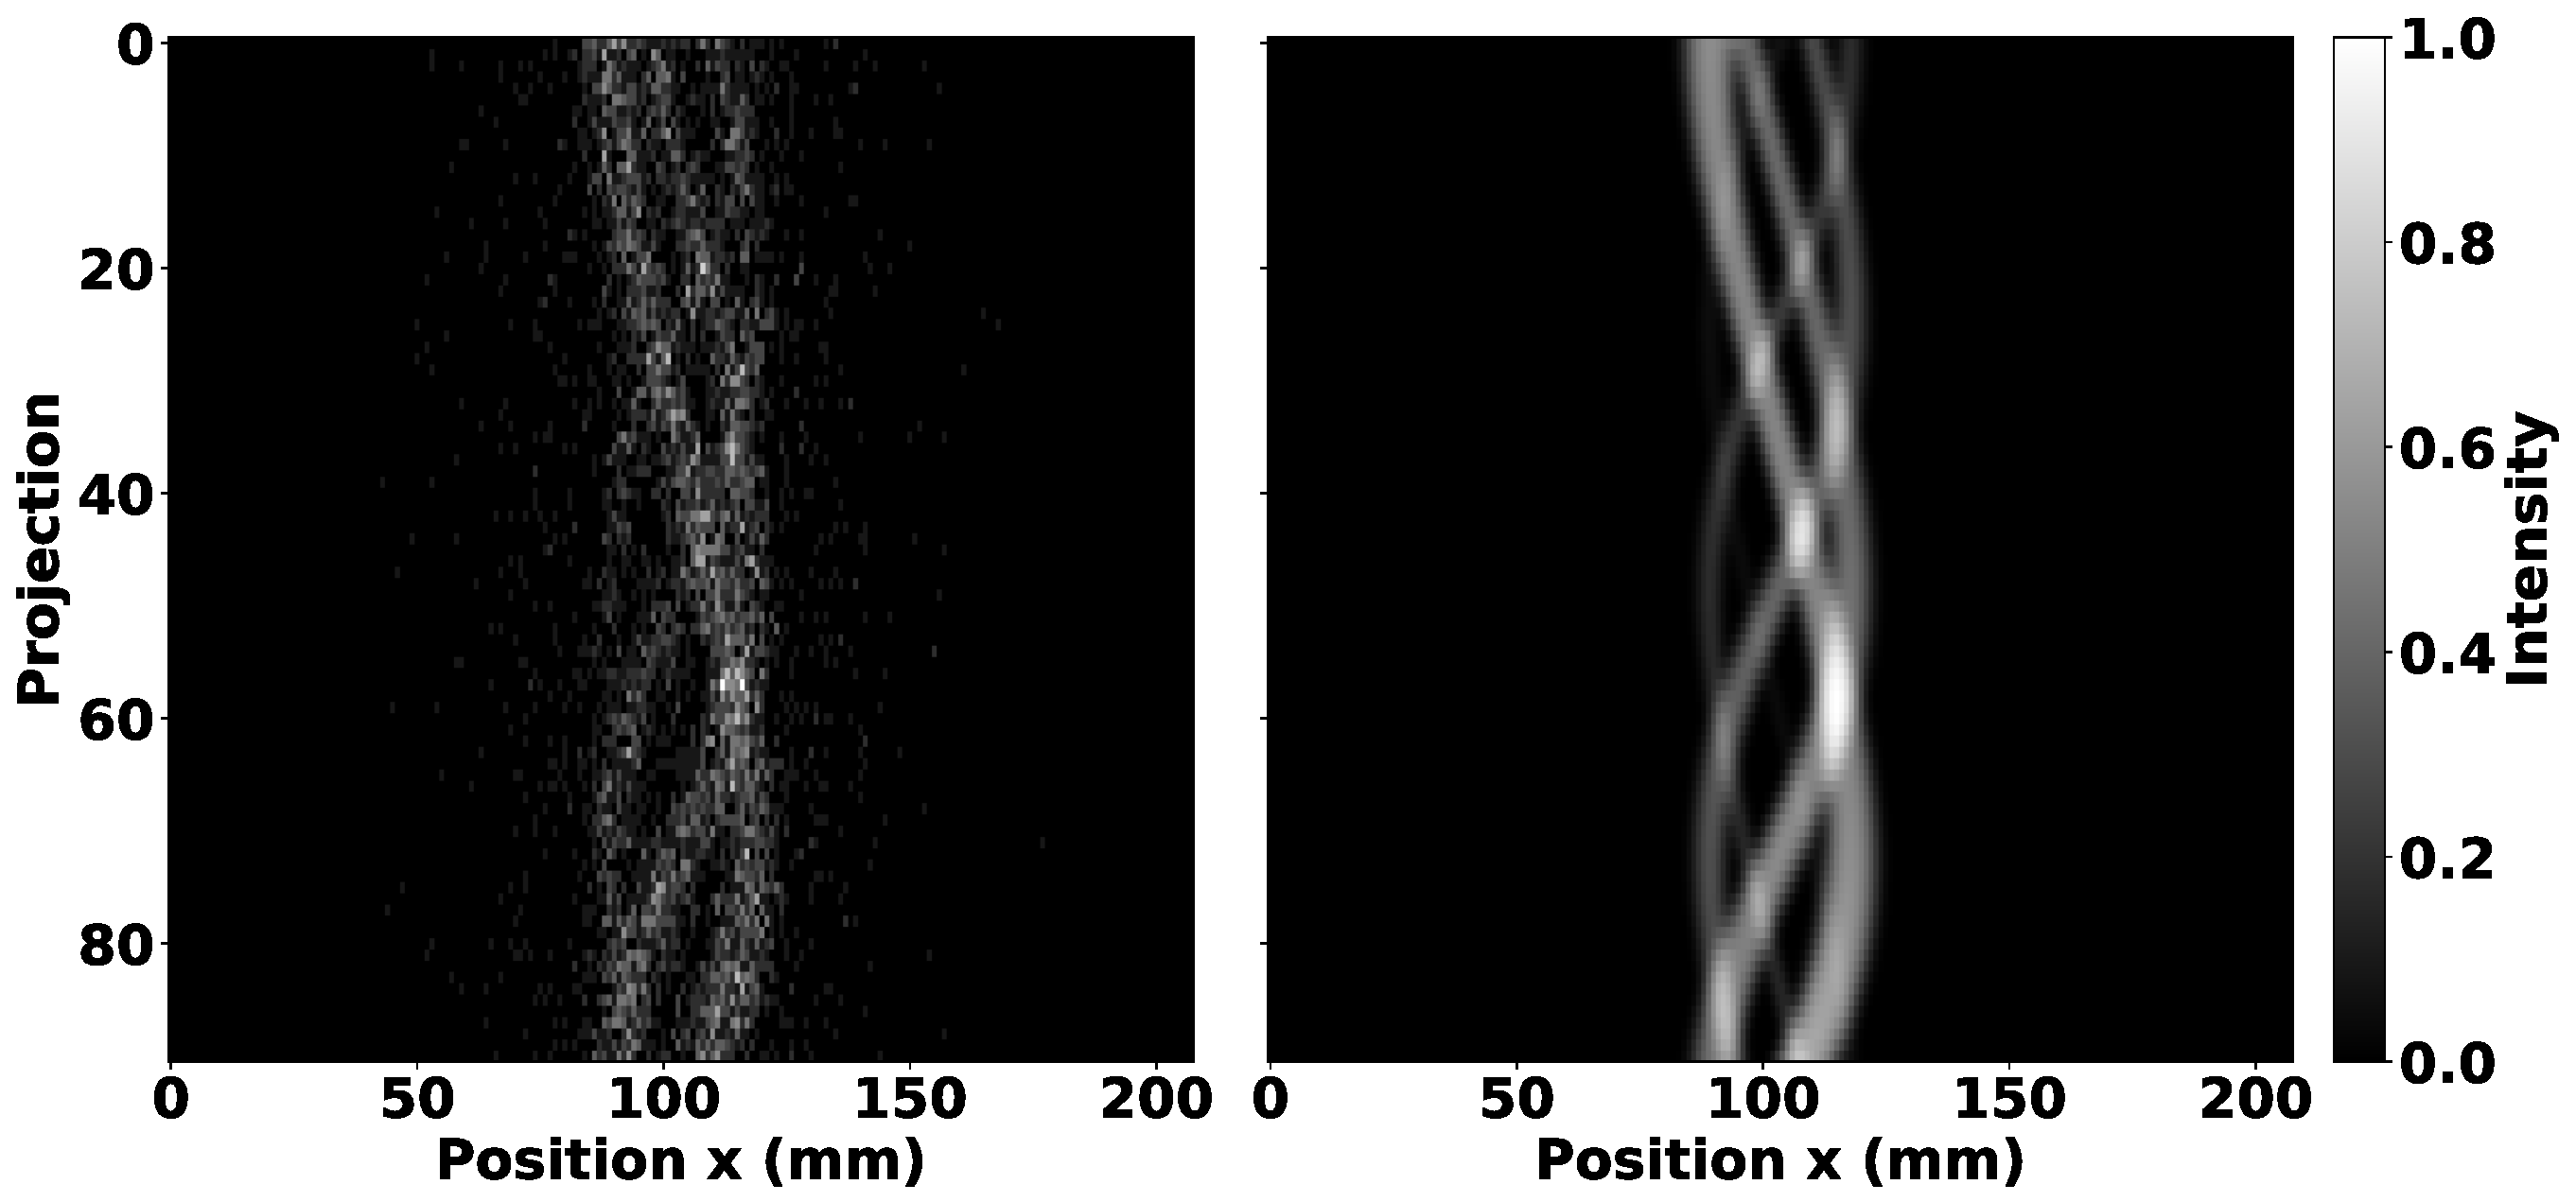
\includegraphics[width=0.71\textwidth]{Figures/HotRod_sinograms_y130}
\end{center}
\caption{Projection of IQ phantom hot rod region displayed in a 2D sinogram arrangement showing the GATE simulated data (\textbf{left}) and the STIR forward projection of the radioactive source distribution adding PSF, DOI, and ATT degradations (\textbf{right}).}
\label{fig:HotRod_sinos}
\end{figure}


%-------------------------------------------------
\begin{figure}[ht!]
	\begin{center}
		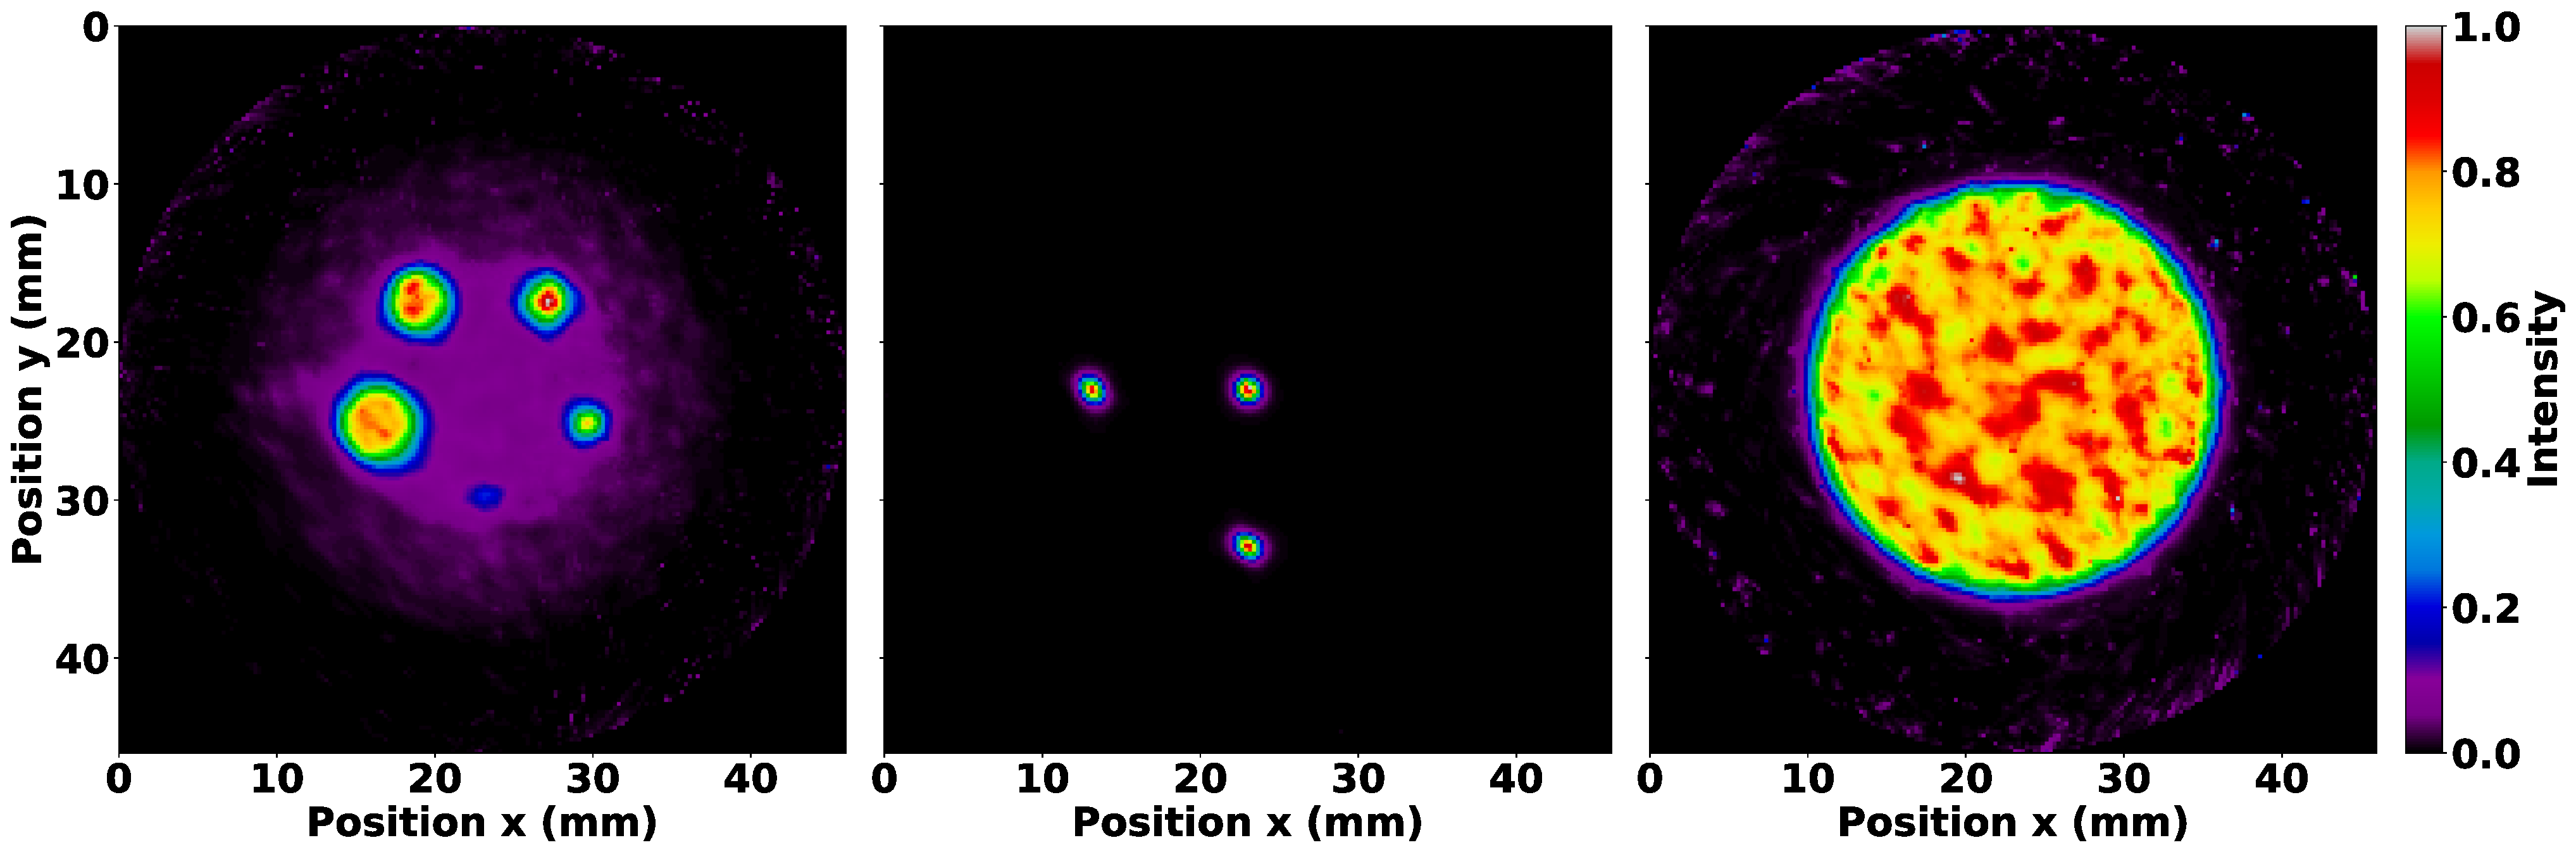
\includegraphics[width=\textwidth]{Figures/OSEM_reconstructions}
	\end{center}
	\caption{Simulated data. Axial sum of normalized OSEM images after 35 subiterations with no matrix corrections and seven subsets for the IQ phantom hot rods (\textbf{left}), mouse-sized NEMA line source phantom (\textbf{middle}), and volumetric cylinder (\textbf{right}). The IQ phantom image was summed over the length of the hot rods whereas the other images were summed over the entire length of the reconstructed image. Note the expected distributions of \ce{^{99m}Tc}.}
	\label{fig:reconstructions}
\end{figure}


%-------------------------------------------------
\begin{figure}[ht!]
\begin{center}
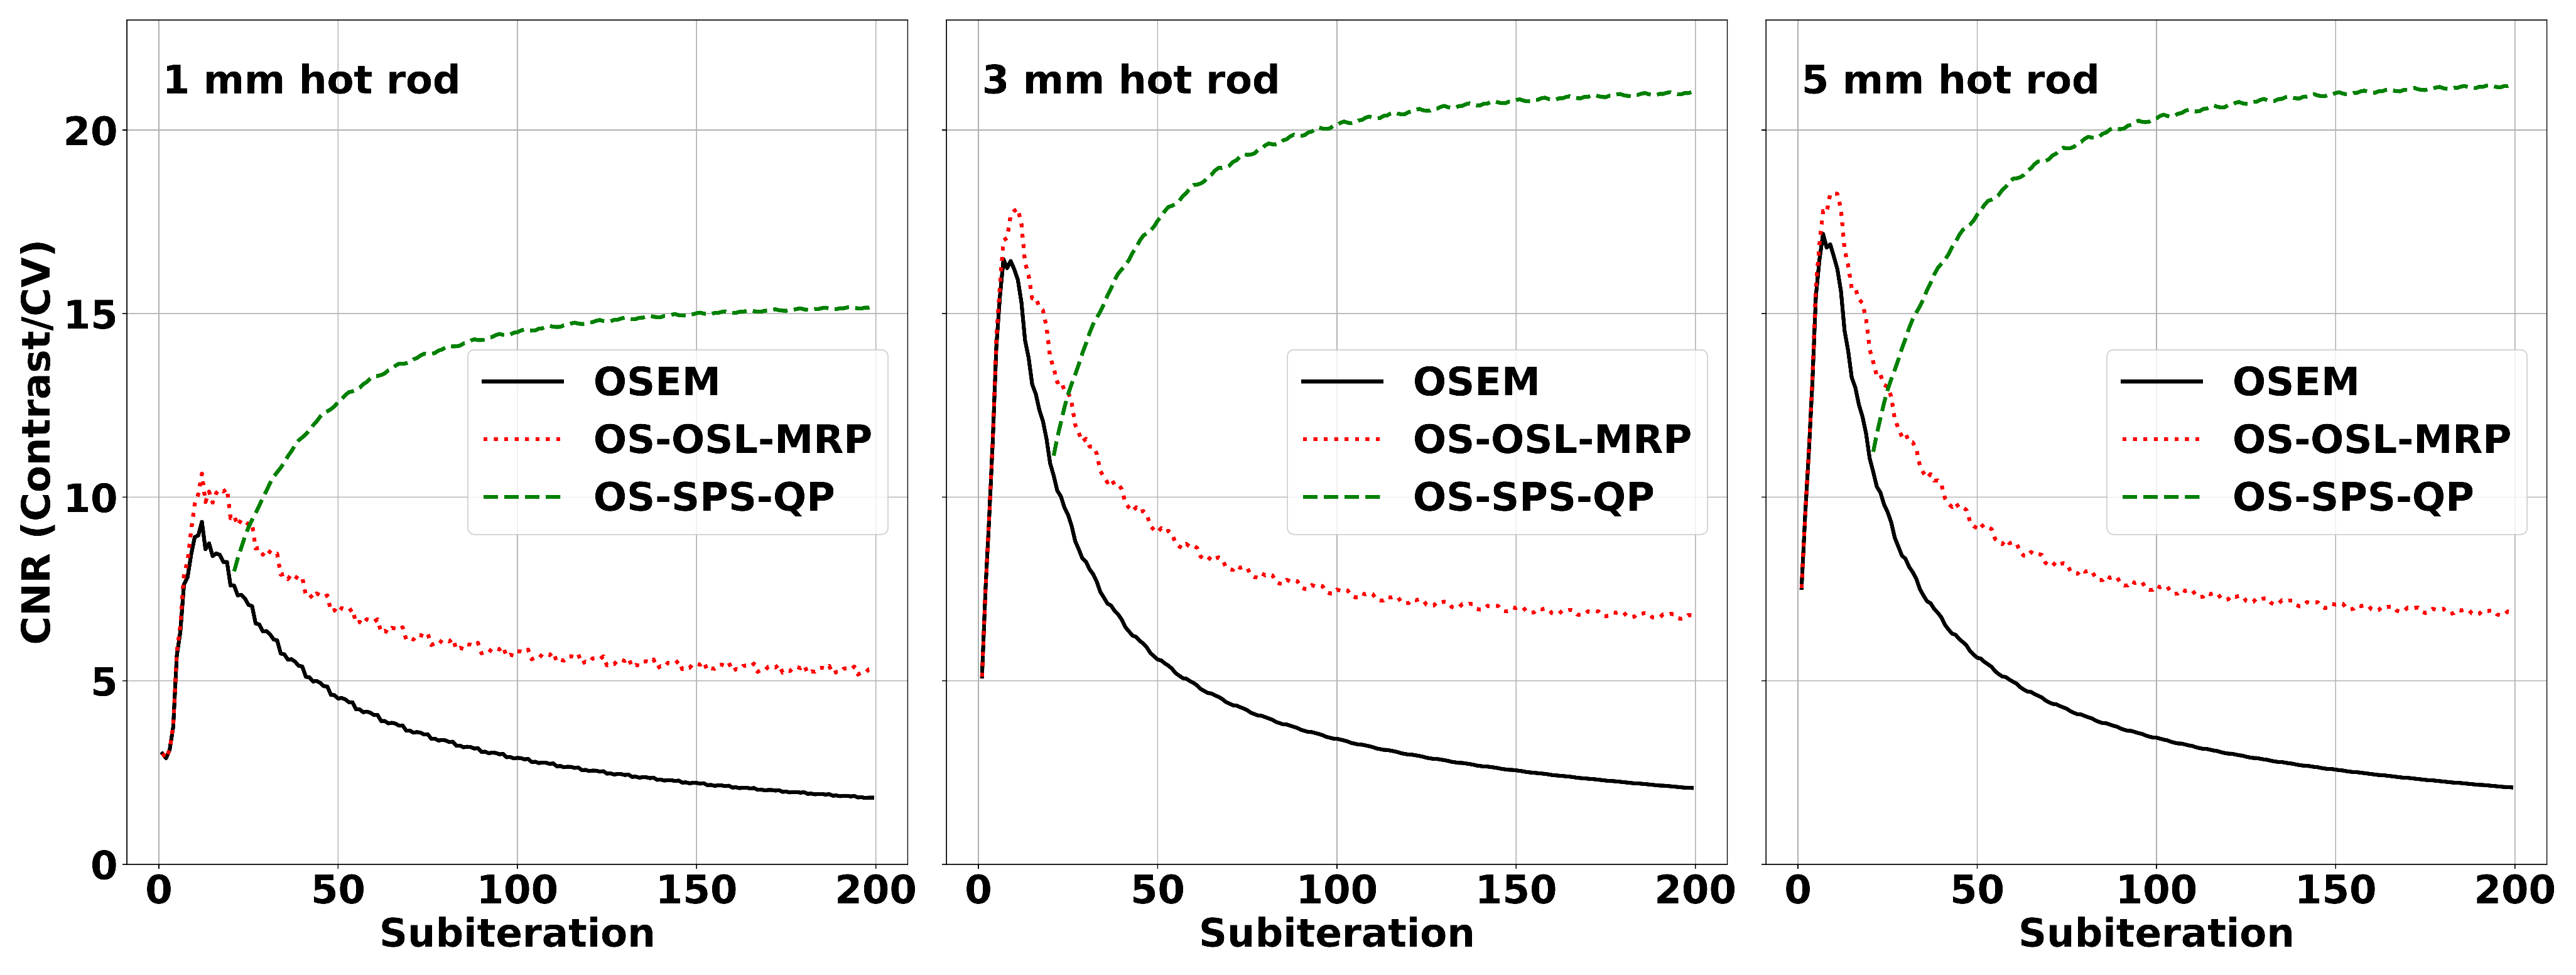
\includegraphics[width=\textwidth]{Figures/HotRod_CNR}
\end{center}
\caption{IQ phantom hot rod CNR plots comparing OSEM (solid line), OS-OSL with median root prior (dotted line), and OS-SPS with quadratic prior (dashed line) over subiterations for the 1 mm hot rod (\textbf{left}), 3 mm hot rod (\textbf{middle}), and 5 mm hot rod (\textbf{right}). All images were reconstructed with no matrix corrections and seven subsets, and the OS-SPS-QP reconstruction was initialized using the OSEM image after 21 subiterations. Hot rod contrast was calculated relative to the central inter-rod region void of \ce{^{99m}Tc}, and CV was calculated in the uniform \ce{^{99m}Tc} region.}
\label{fig:CNR}
\end{figure}


%-------------------------------------------------
\begin{figure}[ht!]
\begin{center}
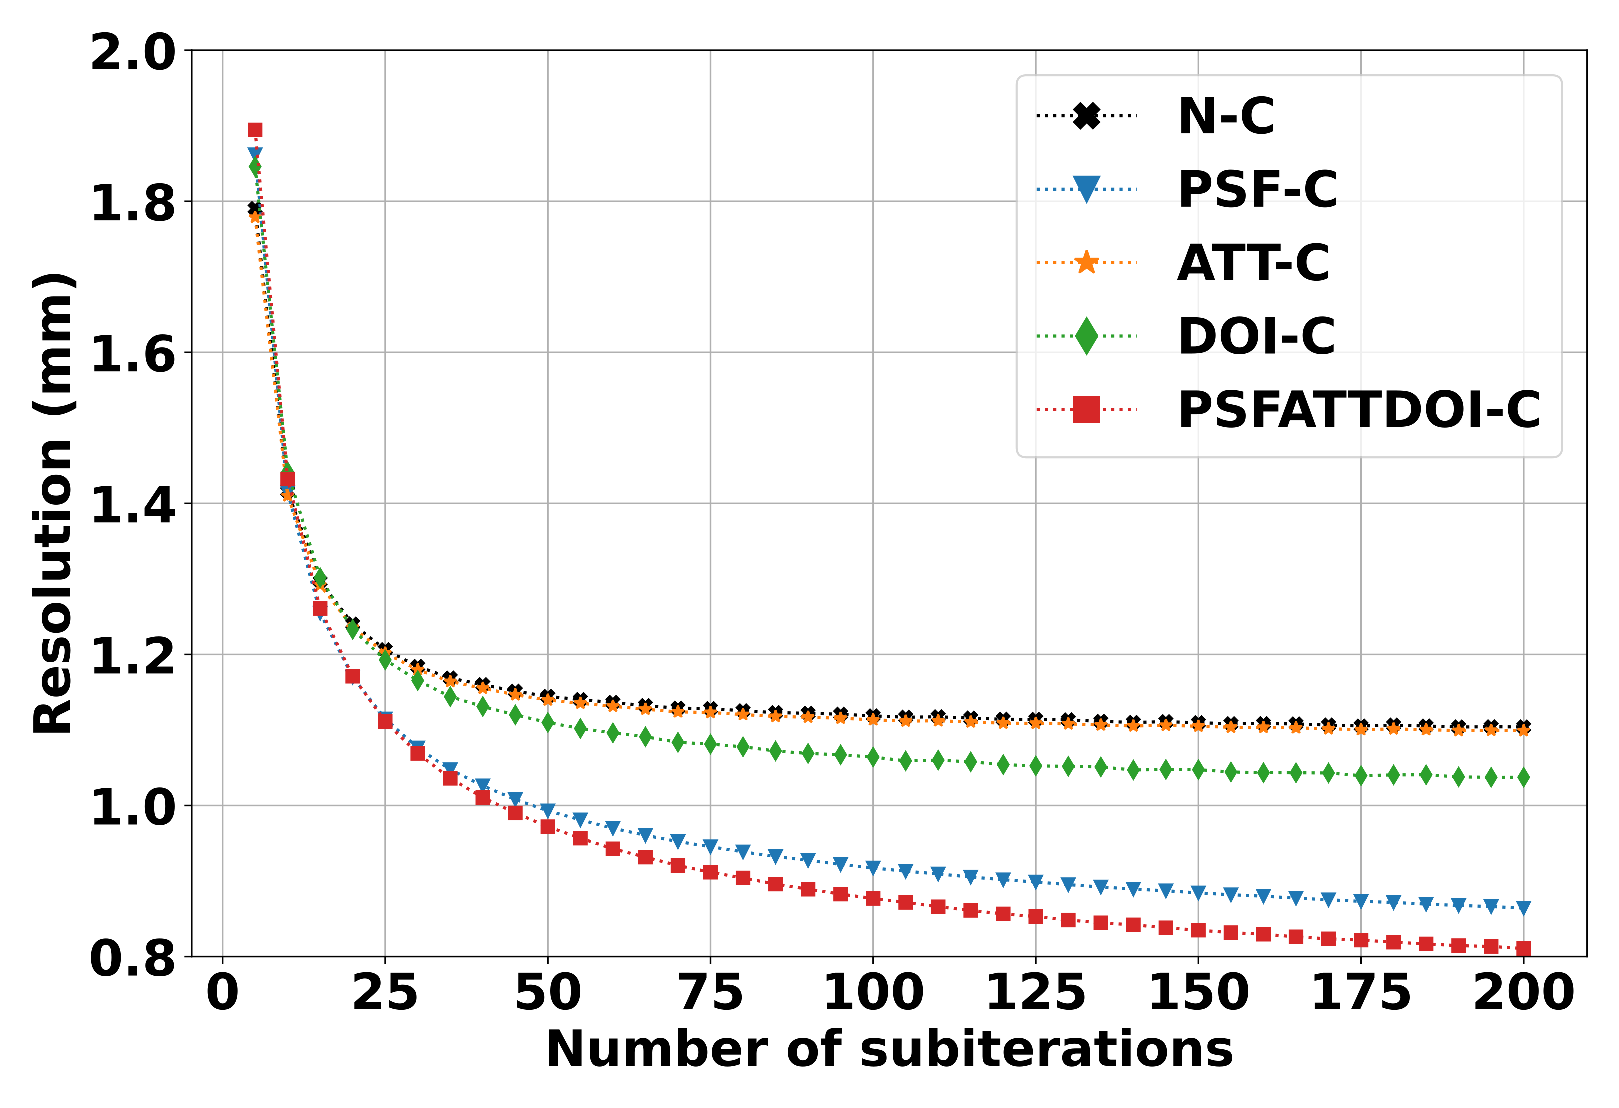
\includegraphics[width=0.49\linewidth]{Figures/Resolution}
\end{center}
\caption{SPECT spatial resolution with scatter in the mouse-sized NEMA triple line source phantom using the OSEM algorithm with seven subsets.}\label{fig:resolution}
\end{figure}


%-------------------------------------------------
\begin{figure}[ht!]
\begin{center}
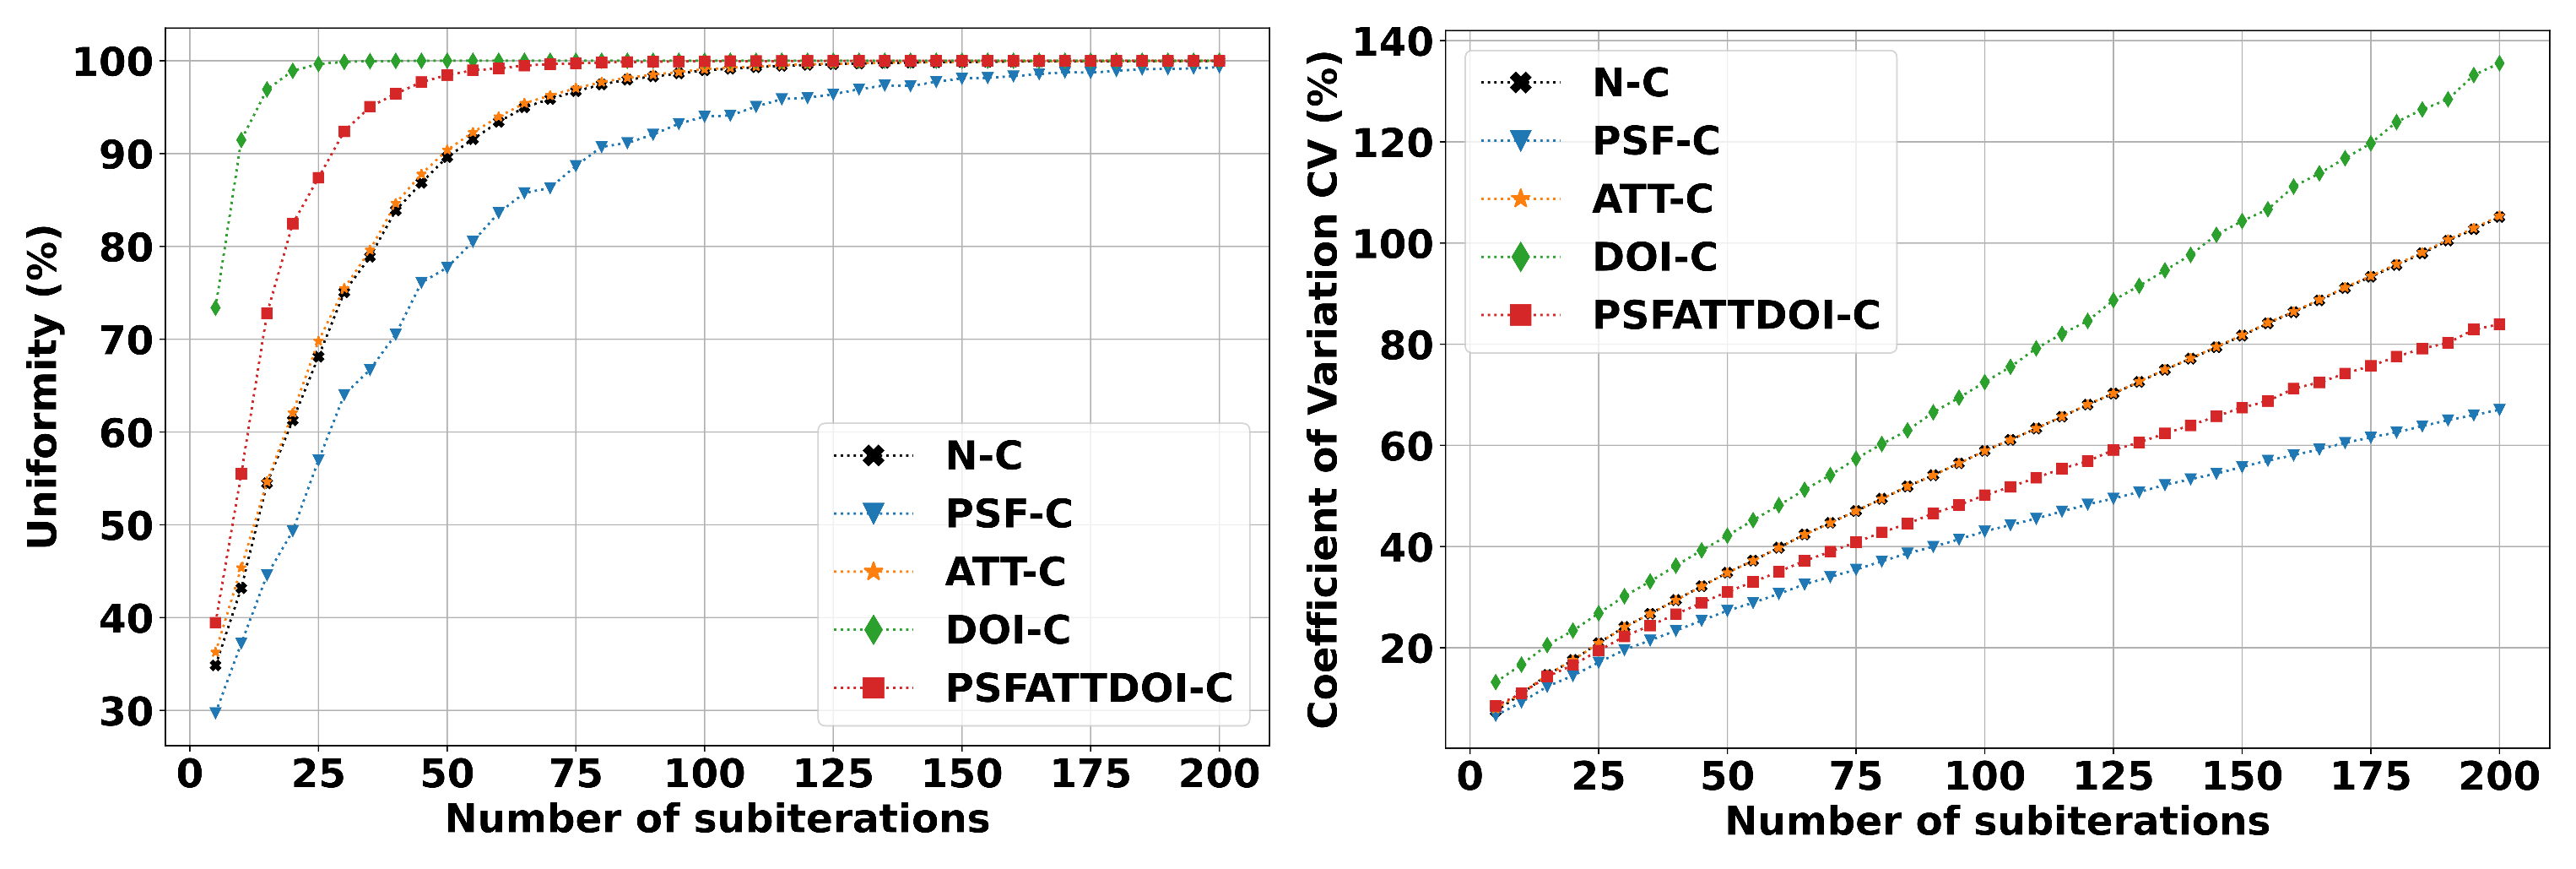
\includegraphics[width=\linewidth]{Figures/Uniformity_Variability}
\end{center}
\caption{SPECT uniformity (\textbf{left}) and variability (\textbf{right}) in the volumetric cylinder using the OSEM algorithm with 7 subsets.}\label{fig:uniformity_variability}
\end{figure}


%-------------------------------------------------
%\begin{figure}
%    \centering
%    \begin{minipage}[t]{0.5\textwidth}
%        \includegraphics[width=\linewidth]{Figures/VSAC_Uniformity.pdf}
%    \end{minipage}%
%    \begin{minipage}[t]{0.5\textwidth}
%        \includegraphics[width=\linewidth]{Figures/VSAC_CV.pdf}
%    \end{minipage}
%\caption{SPECT uniformity (\textbf{left}) and variability (\textbf{right}) in the volumetric cylinder using the OSEM algorithm with 7 subsets.}\label{fig:uniformity_variability}
%\end{figure}


%-------------------------------------------------
\begin{figure}[ht!]
\begin{center}
%\includegraphics[width=0.5\linewidth]{Figures/InVivo.pdf}
\end{center}
\caption{Sagittal fused SPECT/CT of the \textit{in vivo} mouse with a window ranging from 0 to 1. The \ce{^{123}I} distribution shows a nonpersistent tracer in the brain.}\label{fig:invivo}
\end{figure}


%-------------------------------------------------
\begin{figure}[ht!]
\begin{center}
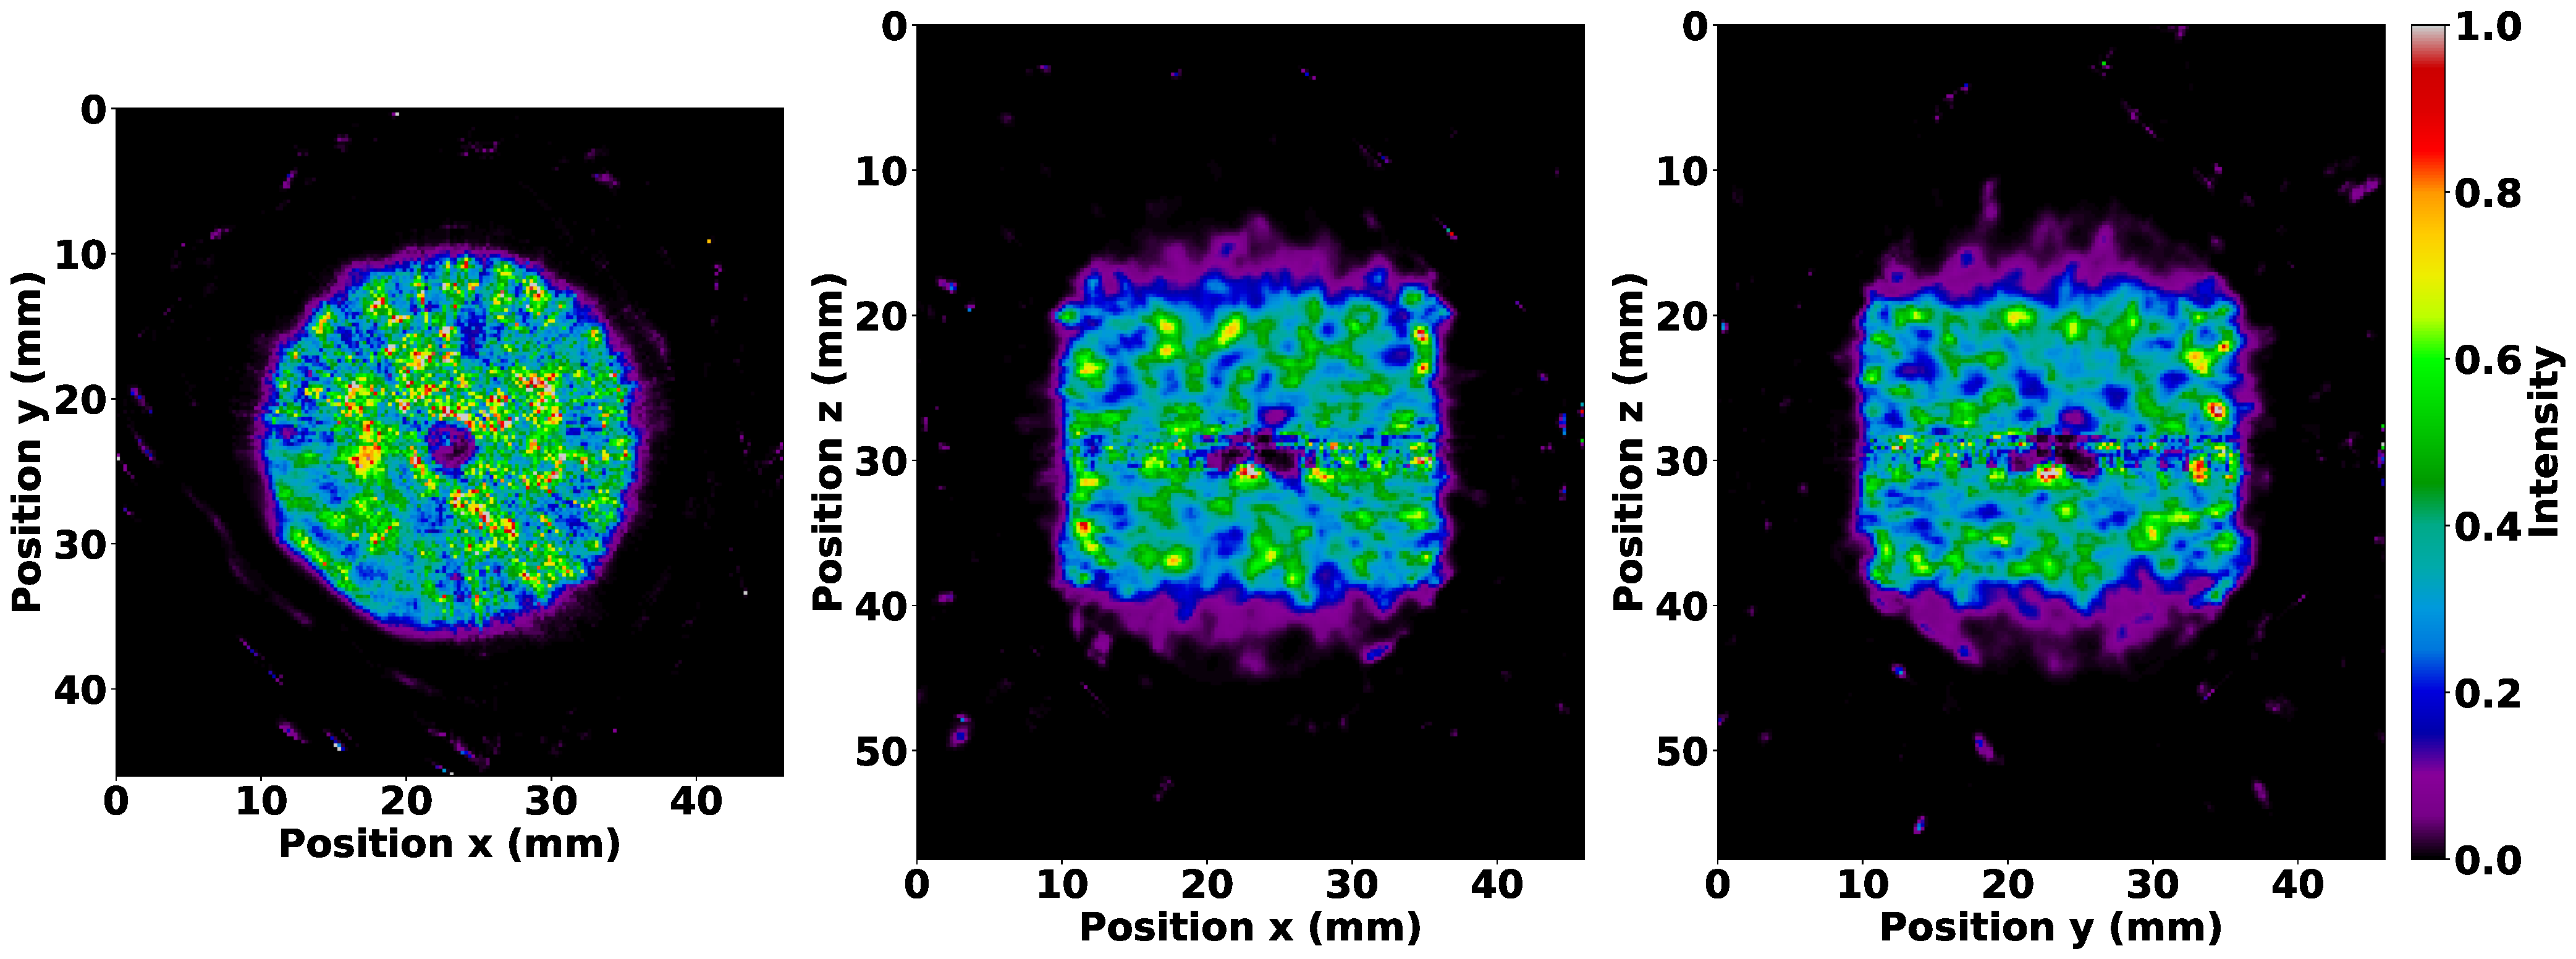
\includegraphics[width=\textwidth]{Figures/DOI_CylVol_bug}
\end{center}
\caption{Slices of the volumetric cylinder reconstructed with OSEM in 35 subiterations using DOI correction where image values were thresholded between 0 and 1. The DOI correction bug is illustrated in the central axial (\textbf{left}), coronal (\textbf{middle}), and sagittal (\textbf{right}) planes. The bug affects voxels within a small angle from the pinhole axis as seen along the pinhole trajectory in a 270 $\deg$ counter-clockwise acquisition starting at 180 $\deg$. The axial view shows the formation of a multi-armed cross or `star shot' artifact, and all views show the compounding effect at the isocenter due to the intersection of LORs affected by the bug.}
\label{fig:DOIbug}
\end{figure}


\end{document}
